\documentclass[aspectratio=169]{beamer}
\usetheme{metropolis}
\usepackage[T1]{fontenc}
\usepackage{booktabs}
\usepackage{graphicx}
\usepackage{tabularx}
\usepackage{tikz}
\usetikzlibrary{arrows.meta,positioning,shapes.geometric}

\metroset{
  progressbar=frametitle,
  numbering=fraction,
  block=fill
}

\definecolor{ILABNavy}{HTML}{071B2F}
\definecolor{ILABBlue}{HTML}{123C69}
\definecolor{ILABOrange}{HTML}{F97316}
\definecolor{ILABGold}{HTML}{FDBA2D}
\definecolor{ILABTeal}{HTML}{13A89E}
\definecolor{ILABInk}{HTML}{142033}
\definecolor{ILABSteel}{HTML}{556270}
\definecolor{ILABLine}{HTML}{D8DEE8}
\definecolor{ILABPaper}{HTML}{F7F8FA}

\setbeamercolor{normal text}{fg=ILABInk,bg=white}
\setbeamercolor{frametitle}{fg=white,bg=ILABNavy}
\setbeamercolor{progress bar}{fg=ILABOrange,bg=ILABLine}
\setbeamercolor{alerted text}{fg=ILABOrange}
\setbeamercolor{block title}{fg=white,bg=ILABBlue}
\setbeamercolor{block body}{fg=ILABInk,bg=ILABPaper}
\setbeamercolor{title separator}{fg=ILABOrange}
\setbeamerfont{frametitle}{size=\Large,series=\bfseries}
\setbeamerfont{title}{size=\Large,series=\bfseries}
\setbeamerfont{subtitle}{size=\large}
\setbeamersize{text margin left=8mm,text margin right=8mm}

\newcommand{\code}[1]{{\ttfamily\detokenize{#1}}}
\newcommand{\pathref}[1]{{\scriptsize\ttfamily\detokenize{#1}}}
\newcommand{\smallpath}[1]{{\tiny\ttfamily\detokenize{#1}}}
\newcommand{\tightsep}{\vspace{0.35em}}
\newcommand{\ok}{\textcolor{ILABTeal}{ready}}
\newcommand{\gated}{\textcolor{ILABOrange}{operator-gated}}
\newcommand{\watch}{\textcolor{ILABGold}{watch}}
\newcommand{\chip}[1]{\begingroup\setlength{\fboxsep}{2pt}\colorbox{ILABOrange!16}{\scriptsize\textcolor{ILABNavy}{#1}}\endgroup}

\newcommand{\dotgrid}[1][ILABOrange!48]{%
  \begin{scope}[shift={(current page.north east)},x=0.18cm,y=0.18cm]
    \foreach \x in {0,...,9} {
      \foreach \y in {0,...,4} {
        \fill[#1] (-4-\x,-3-\y) circle (0.08);
      }
    }
  \end{scope}
}

\newcommand{\sectionframe}[2]{%
  \begin{frame}[plain]
    \begin{tikzpicture}[remember picture,overlay]
      \fill[ILABNavy] (current page.south west) rectangle (current page.north east);
      \fill[ILABOrange] (current page.south west) rectangle ([xshift=0.34cm]current page.north west);
      \draw[ILABOrange,line width=1.2pt] ([xshift=1.1cm,yshift=-1.55cm]current page.north west) -- ++(4.3cm,0);
      \dotgrid[ILABOrange!55]
    \end{tikzpicture}
    \vspace*{1.15cm}
    {\color{ILABOrange}\Large #1\par}
    \vspace{0.55cm}
    {\color{white}\Large\bfseries #2\par}
  \end{frame}
}

\newcommand{\decktitleframe}[4]{%
  \begin{frame}[plain]
    \begin{tikzpicture}[remember picture,overlay]
      \fill[ILABNavy] (current page.south west) rectangle (current page.north east);
      \fill[ILABOrange] (current page.south west) rectangle ([xshift=0.36cm]current page.north west);
      \node[anchor=east,opacity=0.33] at ([xshift=-0.55cm,yshift=-0.25cm]current page.east) {
        \includegraphics[height=0.88\paperheight]{#4}
      };
      \dotgrid[ILABOrange!62]
    \end{tikzpicture}
    \vspace*{0.95cm}
    {\color{ILABOrange}\Large #1\par}
    \vspace{0.35cm}
    {\color{white}\Large\bfseries #2\par}
    \vspace{0.35cm}
    {\color{white!78}\large\parbox{0.58\paperwidth}{#3}\par}
    \vfill
    {\color{white!72}\normalsize pctiope/smart-i-lab-testbed \hfill May 2026\par}
  \end{frame}
}

\tikzset{
  ilabbox/.style={
    draw=ILABLine,
    fill=white,
    rounded corners=2pt,
    align=center,
    minimum height=0.82cm,
    font=\scriptsize
  },
  ilabdark/.style={
    draw=white!28,
    fill=white!7,
    rounded corners=2pt,
    align=center,
    minimum height=0.82cm,
    font=\scriptsize,
    text=white
  },
  ilabstore/.style={
    draw=ILABTeal,
    cylinder,
    shape border rotate=90,
    aspect=0.22,
    fill=ILABTeal!12,
    align=center,
    font=\scriptsize,
    minimum height=1.0cm
  },
  ilabflow/.style={-Latex,draw=ILABOrange,line width=1.1pt},
  ilabthinflow/.style={-Latex,draw=ILABSteel,line width=0.9pt},
  ilablane/.style={draw=ILABLine,fill=ILABPaper,rounded corners=3pt}
}


\title{Smart i-LAB Zone 5}
\subtitle{Applied research overview for robust single-zone occupancy estimation}
\author{pctiope/smart-i-lab-testbed}
\date{May 2026}

\begin{document}

\decktitleframe{Applied Research Overview}{Smart i-LAB Zone 5}{Robust Desk/Zone 5 occupancy estimation with imperfect live lab sensing}{../../../Smart-iLab_DigitalTwin/assets/smart_ilab_3d/Smart_I-LAB_floor3d_room_8_44.jpg}

\begin{frame}[shrink=4]{Problem Motivation}
\begin{columns}[T,onlytextwidth]
\column{0.42\textwidth}
\centering

\includegraphics[width=0.92\linewidth,height=0.25\textheight,keepaspectratio]{../../../zone5_cv_time_features_package/web_app_vite/smart-ilab-zone5/src/assets/hero.png}
\vspace{0.25em}


\includegraphics[width=0.96\linewidth,height=0.18\textheight,keepaspectratio]{../../../zone5_cv_time_features_package/cv_counter/masks/cam1-desk5-mask.png}
\vspace{0.15em}

{\tiny\textcolor{ILABSteel}{Tracked dashboard and Desk 5 ROI assets.}\par}

\column{0.54\textwidth}
\begin{block}{Research setting}
Desk/Zone 5 is a live lab zone, not a clean benchmark. Occupancy evidence
arrives through camera labels, AIR-1 environmental readings, smart-plug power,
mmWave motion state, SEN55 air-quality readings, and time.
\end{block}
\tightsep
\begin{itemize}
  \item Streams can be stale, delayed, partial, or absent while the dashboard must stay useful.
  \item CV labels are a practical proxy for occupancy, but they inherit mask, lighting, and occlusion limits.
  \item A useful model must expose probability, readiness, and source health without committing runtime secrets or snapshots.
\end{itemize}
\end{columns}
\end{frame}

\begin{frame}[shrink=3]{Research Gap}
\begin{columns}[T,onlytextwidth]
\column{0.48\textwidth}
\textbf{What simple approaches miss}
\begin{itemize}
  \item A dashboard can show sensor values without validating an occupancy model.
  \item A single-sensor rule can look stable while ignoring stale upstream data.
  \item A model script can optimize metrics while silently learning missingness patterns.
\end{itemize}

\column{0.48\textwidth}
\begin{block}{Gap addressed here}
\small
The Zone 5 work treats robust occupancy estimation as a multimodal, operationally
gated research problem: noisy CV labels, missing sensor values, mmWave recency,
rolling validation, and live deployment gates must be handled together.
\end{block}
\tightsep
\chip{Multimodal}
\hspace{0.35em}
\chip{Missingness-decoupled}
\hspace{0.35em}
\chip{Operational gates}
\end{columns}
\end{frame}

\begin{frame}{Research Questions}
\begin{enumerate}
  \item Can a Zone 5 model combine environmental, power, mmWave, CV, and time features without treating missingness itself as occupancy evidence?
  \item Can mmWave recency add short-history motion context without target leakage?
  \item Can deployment and promotion gates keep the live service stable while the model contract evolves?
\end{enumerate}
\tightsep
\begin{center}
\parbox{0.84\textwidth}{\centering
\small The deck answers these questions with source-grounded method design, architecture evidence, validation gates, and limitations rather than generated run metrics.}
\end{center}
\end{frame}

\begin{frame}[shrink=4]{System And Method Overview}
\begin{columns}[T,onlytextwidth]
\column{0.48\textwidth}
\textbf{Method}
\begin{itemize}
  \item Build a CV-derived \code{zone_occupied} target in 10-second buckets.
  \item Join AIR-1, power, mmWave, SEN55, and time features into rolling windows.
  \item Preserve raw sensor values while keeping missingness indicators out of model inputs.
  \item Add past-only mmWave recency features for short-history motion context.
  \item Deliver retrained models through staged promotion and live readiness checks.
\end{itemize}

\column{0.48\textwidth}
\centering
\resizebox{0.98\linewidth}{!}{%
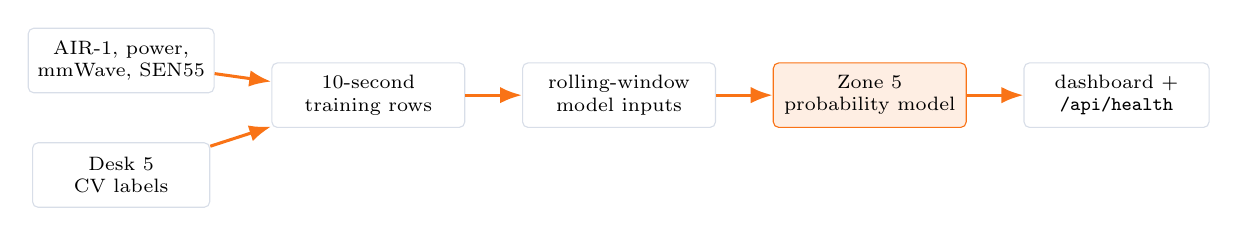
\begin{tikzpicture}[node distance=0.62cm and 0.72cm]
  \node[ilabbox,minimum width=2.25cm] (sensors) {AIR-1, power,\\mmWave, SEN55};
  \node[ilabbox,below=of sensors,minimum width=2.25cm] (cv) {Desk 5\\CV labels};
  \node[ilabbox,right=of sensors,yshift=-0.44cm,minimum width=2.45cm] (table) {10-second\\training rows};
  \node[ilabbox,right=of table,minimum width=2.45cm] (windows) {rolling-window\\model inputs};
  \node[ilabbox,right=of windows,minimum width=2.45cm,fill=ILABOrange!12,draw=ILABOrange] (model) {Zone 5\\probability model};
  \node[ilabbox,right=of model,minimum width=2.35cm] (app) {dashboard +\\\code{/api/health}};
  \draw[ilabflow] (sensors) -- (table);
  \draw[ilabflow] (cv) -- (table);
  \draw[ilabflow] (table) -- (windows);
  \draw[ilabflow] (windows) -- (model);
  \draw[ilabflow] (model) -- (app);
\end{tikzpicture}
}
\tightsep
\begin{block}{Research principle}
\small Model evidence and operational readiness are separated: collection can continue, the dashboard can report health, and promotion can fail without redefining the live API.
\end{block}
\end{columns}
\end{frame}

\begin{frame}[shrink=2]{Technical Architecture As Method Evidence}
\centering
\resizebox{0.98\textwidth}{!}{%
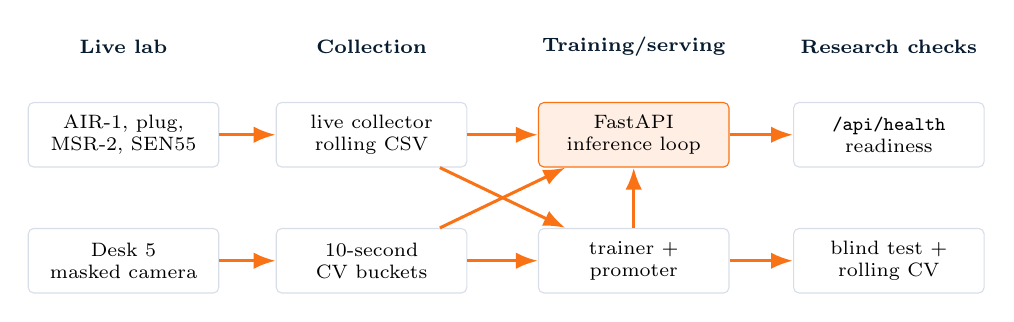
\begin{tikzpicture}[
  node distance=0.70cm and 0.82cm,
  laneTitle/.style={font=\bfseries\scriptsize,text=ILABNavy},
  box/.style={ilabbox,minimum width=2.42cm}
]
  \node[laneTitle] at (0,2.0) {Live lab};
  \node[laneTitle] at (3.15,2.0) {Collection};
  \node[laneTitle] at (6.48,2.0) {Training/serving};
  \node[laneTitle] at (9.72,2.0) {Research checks};

  \node[box] (devices) at (0,0.88) {AIR-1, plug,\\MSR-2, SEN55};
  \node[box] (camera) at (0,-0.72) {Desk 5\\masked camera};
  \node[box] (collector) at (3.15,0.88) {live collector\\rolling CSV};
  \node[box] (aggregator) at (3.15,-0.72) {10-second\\CV buckets};
  \node[box,fill=ILABOrange!12,draw=ILABOrange] (app) at (6.48,0.88) {FastAPI\\inference loop};
  \node[box] (trainer) at (6.48,-0.72) {trainer +\\promoter};
  \node[box] (health) at (9.72,0.88) {\code{/api/health}\\readiness};
  \node[box] (splits) at (9.72,-0.72) {blind test +\\rolling CV};

  \draw[ilabflow] (devices) -- (collector);
  \draw[ilabflow] (camera) -- (aggregator);
  \draw[ilabflow] (collector) -- (app);
  \draw[ilabflow] (aggregator) -- (app);
  \draw[ilabflow] (collector) -- (trainer);
  \draw[ilabflow] (aggregator) -- (trainer);
  \draw[ilabflow] (trainer) -- (app);
  \draw[ilabflow] (app) -- (health);
  \draw[ilabflow] (trainer) -- (splits);
\end{tikzpicture}
}
\tightsep
\begin{center}
\chip{Preserved API surface}
\hspace{0.45em}
\chip{Stable training snapshot}
\hspace{0.45em}
\chip{Promotion before pointer flip}
\hspace{0.45em}
\chip{Runtime state off-source}
\end{center}
\end{frame}

\begin{frame}[shrink=4]{Labeling And Feature Contract}
\begin{columns}[T,onlytextwidth]
\column{0.48\textwidth}
\textbf{Label contract}
\begin{itemize}
  \item Target: \code{zone_occupied}.
  \item Source: Desk 5 CV count aggregated into 10-second buckets.
  \item Positive rule: median \code{occupancy_count} crosses the configured threshold.
  \item Missing CV buckets remain null, not false negatives.
  \item mmWave is an input feature, not the target.
\end{itemize}

\column{0.48\textwidth}
\textbf{Feature contract}
\begin{itemize}
  \item Raw inputs: AIR-1 Zone 5 environment, \code{power_s5}, \code{mmwave_s5}, SEN55, time.
  \item Model contract: \code{zone5_mmwave_recency_v1}.
  \item Missing indicators are retained as diagnostics and metadata, not model inputs.
  \item Core gating covers AIR-1, power, and mmWave; SEN55 is optional and neutral-filled when unavailable.
\end{itemize}
\end{columns}
\end{frame}

\begin{frame}[shrink=3]{mmWave Recency Without Leakage}
\centering
\resizebox{0.95\textwidth}{!}{%
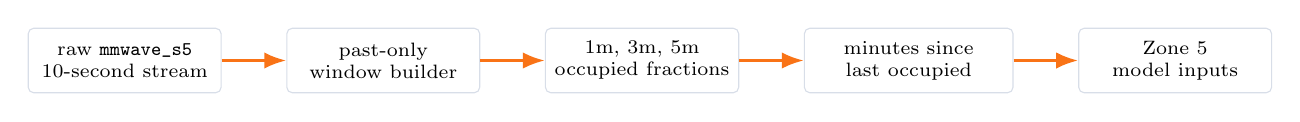
\begin{tikzpicture}[node distance=0.70cm and 0.82cm]
  \node[ilabbox,minimum width=2.45cm] (raw) {raw \code{mmwave_s5}\\10-second stream};
  \node[ilabbox,right=of raw,minimum width=2.45cm] (past) {past-only\\window builder};
  \node[ilabbox,right=of past,minimum width=2.45cm] (frac) {1m, 3m, 5m\\occupied fractions};
  \node[ilabbox,right=of frac,minimum width=2.65cm] (since) {minutes since\\last occupied};
  \node[ilabbox,right=of since,minimum width=2.45cm] (model) {Zone 5\\model inputs};
  \draw[ilabflow] (raw) -- (past);
  \draw[ilabflow] (past) -- (frac);
  \draw[ilabflow] (frac) -- (since);
  \draw[ilabflow] (since) -- (model);
\end{tikzpicture}
}
\tightsep
\begin{columns}[T,onlytextwidth]
\column{0.48\textwidth}
\begin{itemize}
  \item Recency is derived from samples at or before the prediction window.
  \item No future CV label or future mmWave state is allowed into the feature window.
\end{itemize}
\column{0.48\textwidth}
\begin{itemize}
  \item The research question is whether short-history motion improves robustness.
  \item The guard is target separation: \code{zone_occupied} remains CV-derived.
\end{itemize}
\end{columns}
\end{frame}

\begin{frame}[shrink=3]{Evaluation Design And Validation Gates}
\begin{columns}[T,onlytextwidth]
\column{0.48\textwidth}
\textbf{Offline validation}
\begin{itemize}
  \item Hidden blind-test split from the latest calendar day.
  \item Rolling-calendar CV on pre-test dates.
  \item Coverage filtering before strict fold selection.
  \item PR-AUC, ROC-AUC, Brier score, log loss, and both-class checks.
  \item Positive windows, positive buckets, and positive events as evidence gates.
\end{itemize}

\column{0.48\textwidth}
\textbf{Live validation}
\begin{itemize}
  \item Smoke loading verifies target, feature columns, and artifact compatibility.
  \item Same-window non-regression compares candidate and production on the candidate blind-test window.
  \item \code{/api/health} exposes readiness, errors, and model pointer state.
  \item Promotion failure does not stop collectors or dashboard availability.
\end{itemize}
\end{columns}
\end{frame}

\begin{frame}[shrink=3]{Reproducibility And Operational Validity}
\begin{columns}[T,onlytextwidth]
\column{0.48\textwidth}
\begin{block}{Why CI/CD is in the research story}
\small
Model claims are not accepted by source edits alone. Staging, production,
training, and model delivery each have a separate live-exposure gate.
\end{block}
\tightsep
\textbf{Boundaries}
\small
\begin{itemize}
  \item Production: user-systemd live services.
  \item Staging: Docker Compose on separate ports.
  \item Trainer: snapshot, lock, validation, promotion.
  \item Delivery: vetted artifact before pointer update.
\end{itemize}

\column{0.48\textwidth}
\centering
\resizebox{0.94\linewidth}{!}{%
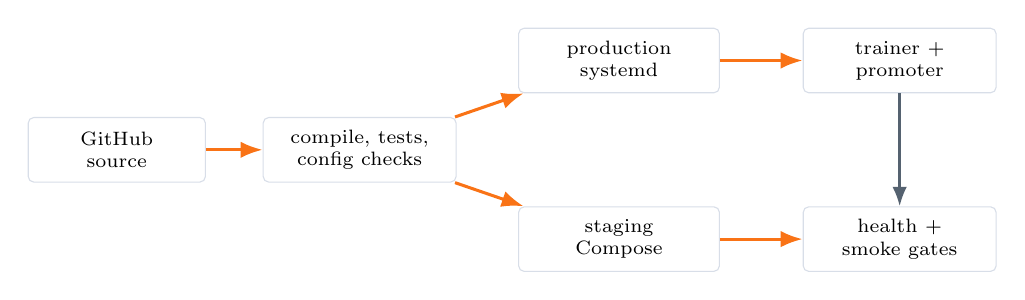
\begin{tikzpicture}[node distance=0.62cm and 0.72cm]
  \node[ilabbox,minimum width=2.25cm] (repo) {GitHub\\source};
  \node[ilabbox,right=of repo,minimum width=2.45cm] (checks) {compile, tests,\\config checks};
  \node[ilabbox,above right=0.30cm and 0.78cm of checks,minimum width=2.55cm] (prod) {production\\systemd};
  \node[ilabbox,below right=0.30cm and 0.78cm of checks,minimum width=2.55cm] (stage) {staging\\Compose};
  \node[ilabbox,right=1.05cm of prod,minimum width=2.45cm] (trainer) {trainer +\\promoter};
  \node[ilabbox,right=1.05cm of stage,minimum width=2.45cm] (health) {health +\\smoke gates};
  \draw[ilabflow] (repo) -- (checks);
  \draw[ilabflow] (checks) -- (prod);
  \draw[ilabflow] (checks) -- (stage);
  \draw[ilabflow] (prod) -- (trainer);
  \draw[ilabflow] (stage) -- (health);
  \draw[ilabthinflow] (trainer) -- (health);
\end{tikzpicture}
}
\end{columns}
\end{frame}

\begin{frame}[shrink=4]{Limitations And Threats To Validity}
\begin{columns}[T,onlytextwidth]
\column{0.49\textwidth}
\textbf{Data and label threats}
\begin{itemize}
  \item CV labels are proxy truth and can fail under occlusion, lighting shifts, or mask errors.
  \item Sensor/API outages can reduce feature coverage or delay joined rows.
  \item Class imbalance and sparse occupied windows can make metrics unstable.
  \item Delayed buckets can revise recent rows after the first live append.
\end{itemize}

\column{0.47\textwidth}
\textbf{Operational threats}
\begin{itemize}
  \item Network reachability and upstream API latency affect live inference freshness.
  \item Artifact compatibility must be explicit as the contract evolves.
  \item A healthy dashboard is not proof that the latest candidate model is valid.
  \item Source docs intentionally exclude populated env values, logs, and run artifacts.
\end{itemize}
\end{columns}
\end{frame}

\begin{frame}[shrink=4]{Research Roadmap And Source Anchors}
\begin{columns}[T,onlytextwidth]
\column{0.42\textwidth}
\textbf{Roadmap}
\begin{itemize}
  \item Continue proving strict rolling-calendar candidates before scheduled retraining is expanded.
  \item Track model freshness, upstream latency, and label coverage as first-class readiness signals.
  \item Keep raw-sensor feature evolution separate from missingness-as-signal regressions.
\end{itemize}

\column{0.54\textwidth}
\tiny
\renewcommand{\arraystretch}{0.96}
\begin{tabularx}{\textwidth}{@{}lX@{}}
\toprule
\textbf{Topic} & \textbf{Primary source paths} \\
\midrule
Pipeline & \pathref{zone5/.../PIPELINE.md} \\
Features & \pathref{zone5/.../feature_contract.py} \\
CV labels & \pathref{zone5/.../build_cv_training_data.py} \\
mmWave recency & \pathref{zone5/.../feature_contract.py} \\
Validation & \pathref{zone5/.../promote_model.py} \\
Gates & \pathref{.github/.../zone5-*.yml}, \pathref{zone5/.../CICD_*.md} \\
\bottomrule
\end{tabularx}
\renewcommand{\arraystretch}{1.0}
\end{columns}
\tightsep
\begin{center}
\parbox{0.82\textwidth}{\centering\textbf{Closing point: Zone 5 treats model contract, labels, and rollout gates as part of the research method.}}
\end{center}
\end{frame}

\end{document}
